\documentclass[12pt]{article}
\usepackage{natbib}
% \usepackage[hypertex]{hyperref}
\usepackage{bm}
\usepackage{amsfonts}
\usepackage{graphicx}


\oddsidemargin 0.0mm
\evensidemargin 0.0mm
\textwidth 160mm
\topmargin -10mm
\textheight 230mm
% \pagestyle{empty}

%%%%%%%%%%%%%%%%%%%%%%%%%%%%%%%%%%%%%%%%%%%%%%%%%%%%%%%%%%%%%%%%%%%

\newcommand{\threej}[6]
{ \left(\begin{array}{ccc}
#1&#2&#3\\
#4&#5&#6
\end{array}\right) }

\newcommand{\sixj}[6]
{ \left\{\begin{array}{ccc}
#1&#2&#3\\
#4&#5&#6
\end{array}\right\} }

\def\separation {0.5cm}
\def\ion#1#2  {#1\,{\small {#2}} }
\def\B{\textsc{BayesCLUMPY}}

%%%%%%%%%%%%%%%%%%%%%%%%%%%%%%%%%%%%%%%%%%%%%%%%%%%%%%%%%%%%%%%%%%%


% For generation of the HTML manual with tth:
% \def\tthdump#1{#1}      % For generating TeX source; ignored by tth
% Redefine symbols problematic for the browser:
%%tth:\def\ga{\hbox{$>\sim$}}
%%tth:\def\la{\hbox{$<\sim$}}
%%tth:\def\Mo{\hbox{$M_o$}}
%%tth:\def\Lo{\hbox{$L_o$}}
%%tth:\def\Mdot{\hbox{$M^{dot}$}}
%%tth:\def\Ivezic{Ivezic}

%%tth:\begin{html}<TITLE>User Manual for MOLPOP-CEP</TITLE>\end{html}
%%tth: This HTML file was generated from the TeX source by
%%tth: the translator TTH, which uses symbol fonts.  These fonts are
%%tth: not normally enabled for Netscape running under X, because of
%%tth: the way Netscape groups its fonts. If your browser has problems
%%tth: displaying the math symbols in this manual, an easy fix can be found
%%tth: on the TTH website at
%%tth:\begin{html}<A HREF="http://hutchinson.belmont.ma.us/tth/Xfonts.html">http://hutchinson.belmont.ma.us/tth/Xfonts.html</A>\end{html}
%%tth:\begin{html}<HR>\end{html}
%%%%%%%%%%%%%%%%%%%%%%%%%%%%%%%%%%%%%%%%%%%%%%%%%%%%%%%%%%%%%%%%%%%

\begin{document}

\title                  {\sc User Manual for \B\footnote{\B\ is one of the IAC computer
programs for synthesizing and making Bayesian inference of spectral energy distributions using the
clumpy dusty torus model of the Kentucky group.}}

\author{ A. Asensio Ramos \\ C. Ramos Almeida\\\\\\
         Instituto de Astrof\'{\i}sica de Canarias\\
         38205, La Laguna, Tenerife, Spain\\
        \\[0.5in] \today}
\date{}
\maketitle

\newpage

\tableofcontents

\newpage

\section*{Disclaimer}

This software is distributed ``as is'' and the authors do not take any responsability for
possible errors derived from its use by others. Apply it with care and
never trust the output without a careful meditation. \B\ can be freely used
provided that its origin is properly acknowledged and the reference Asensio Ramos \& 
Ramos Almeida (2009; ApJ 696, 2075) is cited and acknowledged in any
publication achieved with it. Before using \B\ we recommend the user to read carefully this
paper. Please, 
send us bug reports, comments and suggestions of possible improvements.
We point out that \B\ will be improved over the years, but it is now ready for a number of
interesting applications.

\section*{License}
\emph{This software is Copyright 2009 Andr\'es Asensio Ramos and Cristina Ramos Almeida. The software
may be used for experimental and research purposes only. Commercial use is
not permitted without prior agreement of the Copyright holders. The
software may be shared or distributed under the same restrictions, provided
all such users are made aware of this agreement. The software may not be
sold in whole or within part of a larger software product, whether in
source or binary forms.}

\newpage

%%%%%%%%%%%%%%%%%%%%%%%%%%%%%%%%%%%%%%%%%%%%%%%%%%
%%%%%%%%%%%%%%%%%%%%%%%%%%%%%%%%%%%%%%%%%%%%%%%%%%
\section{Introduction}

\B\ is a computer program that can be used for the fast synthesis of spectral
energy distributions (SED) emerging from clumpy dusty torus models developed by
the Kentucky group. The fast synthesis is accomplished by the usage
of machine learning tools that learn the database of models. These fast
synthesis capabilities are used in a Bayesian scheme for carrying out 
inference over the model parameters for observed SED. Inference can be carried out
with our own Monte Carlo sampler or the MultiNest sampler of Feroz, Hobson \& Bridges 
(2008, arXiv:0809.3437).
The code is written in standard Fortran 90 and IDL. A
front-end coded in IDL is given as a part of the 
distribution in order to facilitate a user-friendly execution of the program.

%%%%%%%%%%%%%%%%%%%%%%%%%%%%%%%%%%%%%%%%%%%%%%%%%%
%%%%%%%%%%%%%%%%%%%%%%%%%%%%%%%%%%%%%%%%%%%%%%%%%%
\section{Uncompressing and compiling \B}

The package comes in a single compressed file \texttt{bayesclumpy.tar.gz}. After
unpacking with \texttt{tar zxvf bayesclumpy.tar.gz}, the \B\ directory
will contain the following subdirectories:

\begin{enumerate}
\item
{\tt FORTRAN} contains the Fortran 90 sources and a makefile that can be used
to build the binary file.
\item
{\tt FILTERS} contains the spectral windows of all the possible filters included in \B. The
file The file {\tt normalizations.dat} in this directory indicates the names of the filters.
\item
{\tt NETWORKS} contains binary files with the weights of the neural networks. This directory is
essential for \B\ and its content should not be modified.
\item
{\tt OBSERVATIONS} is a container for all observed SEDs. An example file is given. 
\item
{\tt MARKOVCHAINS} is the default output directory for the Markov chains and for all the
results of the Bayesian inference.
\item
{\tt MANUAL} contains this manual. 
\end{enumerate}

The code has been tested on Linux platforms using the Intel Fortran
Compiler (\texttt{ifort}) and the GNU \texttt{gfortran} compiler. The compilation 
of the F90 code (in directory \texttt{FORTRAN}) is performed
with the supplied \texttt{makefile}. It is quite simple and easy to modify, and
contains additional comments about compiling. The
default compiler is the \texttt{ifort}, although you can use any other
compiler through the variable \texttt{COMPILER}. Examples for \texttt{ifort}
and \texttt{gfortran} are given. Just uncommment the one you prefer both in the \texttt{makefile}
file in the \texttt{FORTRAN} directory and the \texttt{Makefile} file in the 
\texttt{FORTRAN/NESTED} directory.
In order to obtain the executable file, just type:
\begin{verbatim}
       make lapack
       make nested  
       make
\end{verbatim}
in the directory \texttt{FORTRAN} of \B. After compiling and linking, the executable is copied to the root directory of
\B.

The generated object and module files can be cleaned typing:
\begin{verbatim}
       make clean
\end{verbatim}

%%%%%%%%%%%%%%%%%%%%%%%%%%%%%%%%%%%%%%%%%%%%%%%%%%
%%%%%%%%%%%%%%%%%%%%%%%%%%%%%%%%%%%%%%%%%%%%%%%%%%
\section{Command Line Usage}
\B\ is fundamentally controlled via the IDL graphic user interface. However, it is
possible to control it to do inference through the command line
using the input file \texttt{chain.cfg}.

%%%%%%%%%%%%%%%%%%%%%%%%%%%%%%%%%%%%%%%%%%%%%%%%%
\subsection{\texttt{chain.cfg}}
This file is used to indicate the input parameters for the inference process
carried out using Markov chains if one wants to do it manually. Using the file
provided with the distribution in the present version of \B, we analyze one by one all the inputs.

\begin{verbatim}
# What to do?
2
\end{verbatim}
This indicates the process to do: 1) start a standard MCMC chain, 2) continue a previous chain and 3) do
MultiNest inference.

\begin{verbatim}
# Number of parameters
9
\end{verbatim}
Definition of the number of parameters over which we want to carry out inference. It should
be left to 9 and fix parameters using the priors explained below.

\begin{verbatim}
# Maximum number of iterations
60000
\end{verbatim}
Maximum number of iterations of the Markov chain. This number should be chosen small (around 20000-30000) for
test purposes but should be increased to a much larger number for the final results to produce
better mixed chains.

\begin{verbatim}
# Burn-in [%]
40.0000
\end{verbatim}
Percentage of the Markov chain that is discarded from the beginning to avoid
transients. The value of 40\% is probably too much and something between 20-30\% can be
more appropriate. However, given the speed of the calculation, it is possible to
discard such a large piece of the chain without too much problem.

\begin{verbatim}
# Type of chain (MCMC, SAMPL, PRIO)
'MCMC'
\end{verbatim}
Set to MCMC to carry out inference. Set it to PRIO if you want to sample the prior distribution
for comparing with the posterior distribution. This last option is of reduced interest when
using uniform priors but can be of interest when more complex priors are used.

\begin{verbatim}
# File with observations (only used if MCMC)
'OBSERVATIONS/ngc1386_bayesclumpy.cat'
\end{verbatim}
File with the observed SED.

\begin{verbatim}
# Output chain filename
'MARKOVCHAINS/test'
\end{verbatim}
Name of the output file. Several extensions are added for different outputs.

\begin{verbatim}
# SED (0) or SED+AGN (1)
0
\end{verbatim}
Flag that allows the user to include the spectrum of the AGN. It uses
the spectral shape of Rowan-Robinson (1995).

\begin{verbatim}
# Reddening law
0
\end{verbatim}
It is possible to use four different options at the moment:
\begin{itemize}
 \item 0: no reddening law
 \item 2: Seaton (1979) MW
 \item 3: Fitzpatrick (1986) LMC
 \item 5: Calzetti et al. (2000)
\end{itemize}

\begin{verbatim}
PRIOR INFORMATION
# Information (name, minimum, maximum, type, mu, sigma)
'sigma'  15.0000   75.0000  'U'  0.00000  0.00000
'Y'  5.00000   50.0000  'U'  15.0000  2.50000
'N'  1.00000   15.0000  'U'  0.00000  0.00000
'q'  0.00000   2.00000  'U'  0.00000  0.00000
'tauv'  10.0000   67.0000  'U'  0.00000  0.00000
'angle'  0.00000   90.0000  'U'  85.0000  2.00000
'shift'  0.00000   2.00000  'U'  0.00000  0.00000
'extinction'  0.00000   10.0000  'D'  0.00000  0.00000
'redshift'  0.00000   6.00000  'D'  0.00000  0.00000
\end{verbatim}
The previous lines indicate the name of the parameter and the prior distribution for 
each one. Each line for each parameter shows its minimum and maximum value, the type
of prior and two quantities related to special priors (they are ignored if the prior
does not need them). At the moment, it is possible to 
select between:
\begin{itemize}
 \item Uniform priors (U): the prior probability of the parameter is the same in the interval
   between the maximum and minimum and zero outside the interval.
 \item Dirac delta priors (D): the prior probability of the parameter is zero in all the
   points of the interval except for the point indicated by the additional parameter $\mu$.
   This is a cheap way of fixing parameters to known values.
 \item Gaussian priors (G): the prior probability of the parameter follows a Gaussian shape
   centered at $\mu$ and with standard deviation $\sigma$.
\end{itemize}

%%%%%%%%%%%%%%%%%%%%%%%%%%%%%%%%%%%%%%%%%%%%%%%%%
\subsection{Execution}
\label{sec:execution}
After the \texttt{chain.cfg} file is set, the code is run by invoking
\begin{verbatim}
./clumpy_mcmc
\end{verbatim}
After the code is executed, output files are generated. These files are discussed in the
next section. Since the inference is done through a Markov Chain Monte Carlo calculation,
it can suffer from convergence problems. While running, the code prints the average value
of the parameters, together with the estimated standard deviation. An example of the
output is given below:
\begin{scriptsize}
\begin{verbatim}
  9600  Acc. rate:   6.51- 25.50% -- (alp,alp/th):     0.026     0.037 -- logL(max):   -0.5590E+02    
    Avg:     65.4995   41.9076   14.3619    1.2772   35.2157    2.2846    0.1384    0.0612            
    Sigma:    3.1149   12.3222    0.5093    0.1394   10.2167    1.7097    0.0516    0.6019            
  9700  Acc. rate:   6.67- 23.50% -- (alp,alp/th):     0.026     0.037 -- logL(max):   -0.5590E+02    
    Avg:     65.5310   41.9836   14.3495    1.2759   35.1415    2.2872    0.1387    0.0605            
    Sigma:    3.1143   12.2812    0.5213    0.1393   10.1901    1.7021    0.0514    0.5988            
  9800  Acc. rate:   6.78- 19.50% -- (alp,alp/th):     0.026     0.037 -- logL(max):   -0.5590E+02    
    Avg:     65.5597   42.0565   14.3365    1.2740   35.0663    2.2894    0.1390    0.0599            
    Sigma:    3.1122   12.2396    0.5343    0.1399   10.1651    1.6939    0.0512    0.5958
\end{verbatim}
\end{scriptsize}
A standard way to estimate if the Markov chain is in the good direction is to have
an local acceptance rate (the second number after \texttt{Acc. rate:}) in the range 20-30\%.
Another good feeling can be obtained from the value of the logarithm of the posterior (\texttt{logL(max)}).
If this number (normalized to the number of points) is of the order of 1, the Markov chain has
located the regions of high probability and good results should be expected. In case this does
not occur, stop the run and re-run it until the previous conditions are fulfilled.

It is possible to use IDL to quickly synthesize SEDs. For this, enter IDL and do:
\begin{verbatim}
IDL> .r bayesclumpy
IDL> restore,'neural.idl'
IDL> sed = neural_SED(neural, sigma, Y, N, q, tauv, angle, $
     include_agn=include_agn, jansky=jansky, out_agn = out_agn)
\end{verbatim}
\texttt{sigma, Y, N, q, tauv, angle} are the parameters of the clumpy torus model. It returns
the SED that you can plot vs. wavelength with:
\begin{verbatim}
IDL> plot, neural.lambda, sed
\end{verbatim}
The \texttt{include\_agn} parameter is used to include the AGN emission. The \texttt{jansky} flag is 
used to make the output be returned in Jy and \texttt{out\_agn} can be used to return from
the function the AGN spectrum.

%%%%%%%%%%%%%%%%%%%%%%%%%%%%%%%%%%%%%%%%%%%%%%%%%
\subsection{Output files}
\label{sec:output}

\subsubsection{Standard MCMC}
Every run of the \B\ code generates three files with different extensions. The root
of each file is the one selected in the \texttt{chain.cfg} file and the following
extensions are added:
\begin{itemize}
 \item \texttt{.chain}: this is a binary file that contains the Markov chain for all the parameters.
 \item \texttt{.hist1D}: this is a binary file that contains the one-dimensional marginal histograms
   for each parameter.
 \item \texttt{.confidence}: this is a text file that contains information on the retrieved parameters.
 Each line contains the estimated marginal median value, together with the confidence interval at 68\%
 and 95\% confidence, with the lower limit before the upper limit. The last line contains the set of
 parameters that produce the largest value of the full posterior distribution (if all the parameters
 have a uniform prior, this set of parameters coincides with the ones retrieved with a standard 
 least-squares minimization).
\end{itemize}

The IDL program \texttt{readchain.pro} can be used to read the full output. Just invoke it
with \texttt{readchain, 'test'} and it generates the variable \texttt{chains} with the Markov chains,
together with some summarize information about the parameters. It also plots the 1D marginal histograms
for each variable.

\subsubsection{MultiNest}
An additional set of files is generated if MultiNest inference is carried out. The Markov chains
are saved in the file with the extension \texttt{post\_equal\_weights.dat} and the summary
is saved in the file with the extension \texttt{stats.dat}.

%%%%%%%%%%%%%%%%%%%%%%%%%%%%%%%%%%%%%%%%%%%%%%%%%%
%%%%%%%%%%%%%%%%%%%%%%%%%%%%%%%%%%%%%%%%%%%%%%%%%%
\section{Observations}
\label{sec:observations}
The observations are usually saved in the \texttt{OBSERVATIONS} directory. The structure
of the file is as follows:

\begin{verbatim}
'NGC XXXX'
\end{verbatim}
Name of the galaxy for identification purposes.

\begin{verbatim}
3
\end{verbatim}
Number of points of the SED in filter photometry.

\begin{verbatim}
'F160W'         flux1    error1
'trecsN'        flux2    error2
'trecsQa'       flux3    error3
\end{verbatim}
Data for the photometry. Each line indicates a filter (see file \texttt{FILTERS/normalizations.dat'} for
a list of available filters), the flux in mJy and the error as the 68\% confidence interval
assumed symmetric. It is possible to give detection limits by putting the flux in negative (the
absolute value is used in the code) and giving the confidence (0.68, 0.95, etc.) in the second
column.


%%%%%%%%%%%%%%%%%%%%%%%%%%%%%%%%%%%%%%%%%%%%%%%%%%
%%%%%%%%%%%%%%%%%%%%%%%%%%%%%%%%%%%%%%%%%%%%%%%%%%
% \begin{figure}
% \includegraphics[width=\columnwidth]{f5.eps}
% \caption{Screen dump of the graphical front-end used for the synthesis.
% \label{fig:synthesis_GUI}}
% \end{figure}

\section{Graphical front-ends}
Although the code can be run in command line by modifying by hand the input file, 
\B\ contains also a user friendly front-ends (GUI) for the simple execution and
analysis of the results. It is easily executed in IDL by entering:
\begin{verbatim}
IDL> .r bayesclumpy
IDL> bayesclumpy
\end{verbatim}
If errors appear when starting the GUI, use \texttt{bayesclumpy,/reset}.

\begin{figure}[!t]
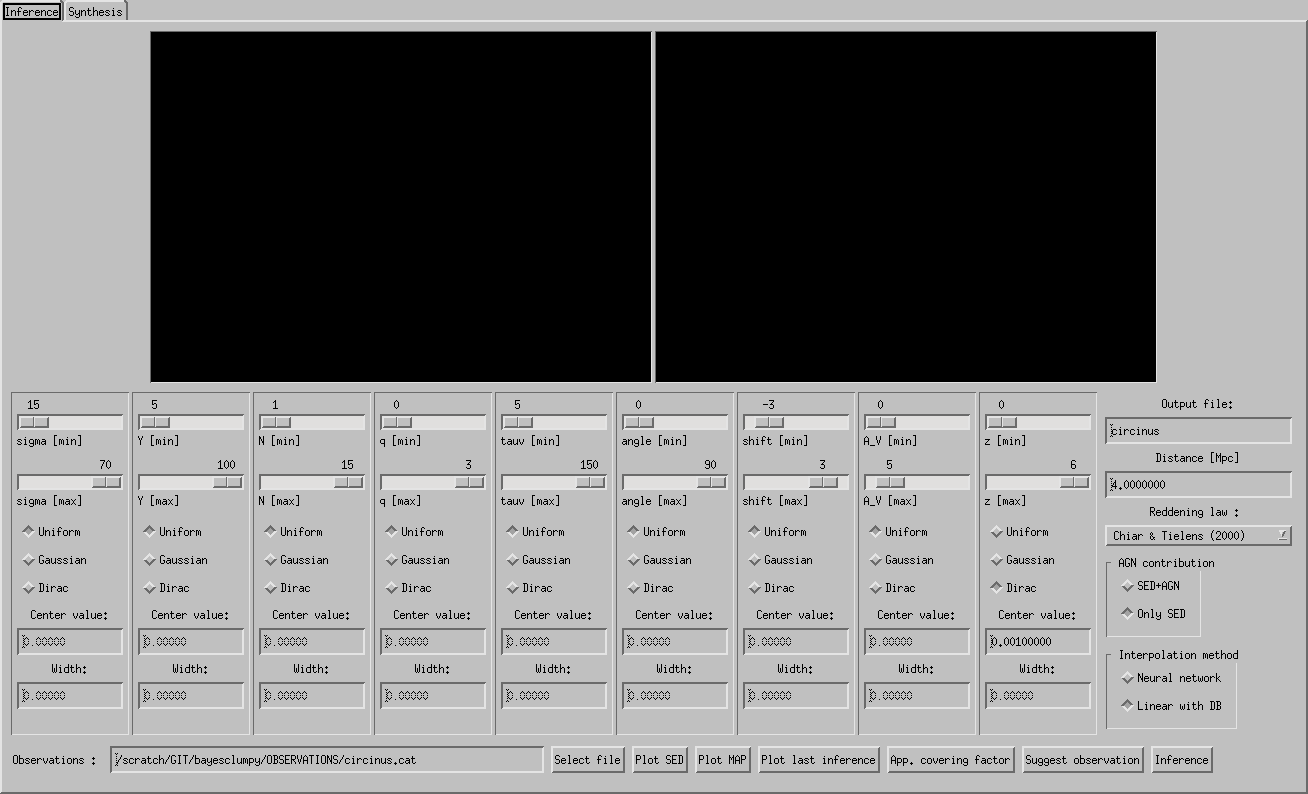
\includegraphics[scale=0.5]{snapshot1.png}
\caption{Screen dump of the graphical front-end used for the inference.
\label{fig:inversion_GUI}}
\end{figure}

\subsection{Inference}
This is the default tab when running the GUI. A snapshot is shown in Fig. \ref{fig:inversion_GUI}.
It can be used to visually change the
parameters defined for the file \texttt{chain.cfg} and execute the inference. It can
also be used to draw the observed SED (``Plot SED'' button), the 1D marginal posterior
distributions obtained in the last inference run (``Plot last inference'' button) and the
SED plus the maximum-a-posteriori fit with the error bars (``Plot MAP'' button). Finally,
the ``Inference button'' runs the code.

\begin{figure}[!t]
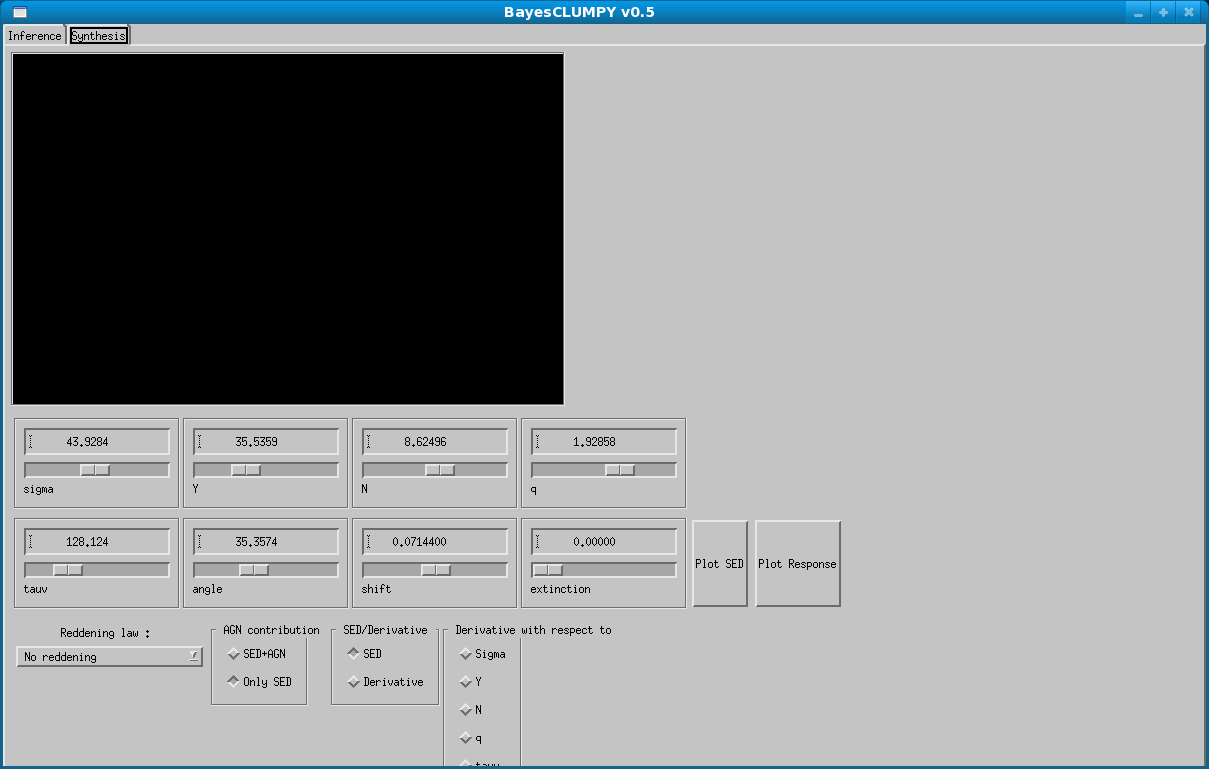
\includegraphics[scale=0.5]{snapshot2.png}
\caption{Screen dump of the graphical front-end used for the synthesis.
\label{fig:synthesis_GUI}}
\end{figure}

\subsection{Synthesis}
This is the GUI that allows the user to synthesize SEDs for any combination of the model
parameters. It is also possible to see the behavior of the response functions (derivative
of the SED at each wavelength with respect to any parameter).

\section{MultiNest License}

MultiNest v 2.7 is used in this version of \B. MultiNest has the following license agreement.

\emph{This software is Copyright 2009 Farhan Feroz and Mike Hobson. The software
may be used for experimental and research purposes only. Commercial use is
not permitted without prior agreement of the Copyright holders. The
software may be shared or distributed under the same restrictions, provided
all such users are made aware of this agreement. The software may not be
sold in whole or within part of a larger software product, whether in
source or binary forms.}


\section*{Acknowledgements}
Finantial support by
the Spanish Ministry of Education and Science through projects AYA2007-63881, AYA2007-67965-C03-01,
the European Commission through the SOLAIRE network (MTRN-CT-2006-035484) and the
Spanish MEC under the Consolider-Ingenio 2010 Program grant CSD2006-00070 is gratefully acknowledged. 

% \bibliographystyle{apj}
% \bibliography{/home/aasensio/biblio}

\end{document}
